
\red{
we use the SUNSET code to perform combustion simulations [cite]

here are explanations of the methods used therein
}


\section{LABFM}

\cite{king2024MeshFreeFrameworkHighOrder, king2020HighOrderDifference, king2024MeshfreeFrameworkHighorder, king2022HighorderSimulationsIsothermal, king2024SunsetFlamesDNSCode}


\subsection{High-Order Interpolations}

% in keeping with other methods, where interpolation is the first step to gradient approximations

Before considering gradient approximations, we choose first to consider interpolations, to make clear the method. We consider a location $\vec{x}$ surrounded locally by finitely many nodes $\vec{x}_j \in \cl{S}(\vec{x})$ which are enumerated by $j \in \cl{N}(\vec{x})$, where $\abs{\vec{x} - \vec{x}_j} < h(\vec{x})$. Assume the function $\phi = \phi(\vec{x})$, which is only known at the points $\phi_j = \phi(\vec{x}_j)$, is \emph{smooth enough}.\footnote{Such that as many derivatives of $\phi$ as are used in the derivation below are available to us.} Then, we express the interpolated value $\phi(\vec{x})$ as a linear combination of the surrounding values $\phi_j$:
\begin{equation} \label{eqn:L}
L^{\rm{int}}[\phi](\vec{x}) \equiv \sum_{j \in \cl{N}(\vec{x})} \phi_j w^{\rm{int}}(\vec{x}, \vec{x}_j) \approx \phi(\vec{x}).
\end{equation}
To find the weights $w^{\rm{int}}(\vec{x}, \vec{x}_j)$, we will be evaluating $\phi_j$ by means of Taylor series via derivatives of $\phi$. Each derivative is a projection from the vector of derivatives of $\phi$:
\begin{equation}
\vv{D}[\phi] = \left(\phi, \pdv{\phi}{x}, \pdv{\phi}{x}, \pdv[2]{\phi}{x}, \pdv[2]{\phi}{x}{y}, \pdv[2]{\phi}{x}, \dots \right)^T
\quad \text{and} \quad
\vv{D}_k[\phi] = \left(\phi, \pdv{\phi}{x}, \pdv{\phi}{x}, \dots, \pdv[k]{\phi}{x}, \dots, \pdv[k]{\phi}{y} \right)^T,
\end{equation}
where we have assumed that $\phi$ is a scalar field over two spatial dimensions $\vec{x}=(x, y)$, although the method may be simply extended to any number of dimensions (with the caveat that the number of nodes required increases greatly with dimension). In this notation, interpolation becomes $\phi(\vec{x}) = \vv{D}[\phi](\vec{x}) \cdot \vv{C}^{\rm{int}} = \vv{D}_k[\phi](\vec{x}) \cdot \vv{C}_k^{\rm{int}}$ where $\vv{D}[\phi](\vec{x})$ is the vector $\vv{D}[\phi]$ evaluated at the location $\vec{x}$, $\vv{C}^{\rm{int}} = (1, 0, 0, 0, 0, 0, \dots)^T$ and $\vv{C}_k^{\rm{int}} = (1, 0, 0, \dots, 0)^T$, is of the same length as $\vv{D}_k$. Introducing the vectors of monomials:
\begin{equation}
\vv{X}(\vec{x}) = \left(1, x, y, \frac{1}{2!} x^2, xy, \frac{1}{2!} y^2, \dots \right)^T
\quad \text{and} \quad
\vv{X}_k(\vec{x}) = \left(1, x, y, \dots, \frac{1}{k!} x^k, \dots, \frac{1}{k!} y^k \right)^T,
\end{equation}
we can simplify down the Taylor expansion of $\phi$ around the point $\vec{x}$ for any $\vec{x}_j$ as:
\begin{subequations}
\begin{align}
\phi_j &= \phi(\vec{x}) + \pdv{\phi}{x}\bigg|_{\vec{x}} (x_j - x) + \pdv{\phi}{y} \bigg|_{\vec{x}} (y_j - y)  \\
& \qquad  \quad \ \, + \frac{1}{2!} \pdv[2]{\phi}{x}\bigg|_{\vec{x}} (x_j - x)^2 + \pdv[2]{\phi}{x}{y}\bigg|_{\vec{x}} (x_j - x) (y_j - y) + \frac{1}{2!} \pdv[2]{\phi}{y}\bigg|_{\vec{x}} (y_j - y)^2 + \dots \\
&= \vv{D}[\phi](\vec{x}) \cdot \vv{X} (\vec{x}_j - \vec{x}),
\end{align}
\end{subequations}
which may be truncated to $\phi_j \approx \vv{D}_k[\phi](\vec{x}) \cdot \vv{X}_k (\vec{x}_j - \vec{x})$ with $\cl{O}(h^{k + 1})$ truncation error. Rewriting \equ{eqn:L} in this formulation:
\begin{subequations}
\begin{align}
L^{\rm{int}}[\phi](\vec{x}) &= \vv{D}[\phi](\vec{x}) \, \cdot \sum_{j \in \cl{N}(\vec{x})} \vv{X} (\vec{x}_j - \vec{x}) w^{\rm{int}}(\vec{x}, \vec{x}_j) \\
&\approx \vv{D}_k[\phi](\vec{x}) \, \cdot \sum_{j \in \cl{N}(\vec{x})} \vv{X}_k (\vec{x}_j - \vec{x}) w^{\rm{int}}(\vec{x}, \vec{x}_j) \equiv \vv{D}_k[\phi](\vec{x}) \cdot \vv{B}_k^\rm{int}(\vec{x}) \\
&\approx \vv{D}_k[\phi](\vec{x}) \cdot \vv{C}_k^{\rm{int}}
\end{align}
\end{subequations}
So our problem now involves finding the correct values of $w^{\rm{int}}(\vec{x}, \vec{x}_j)$ such that the \emph{vector of moments} $\vv{B}_k^{\rm{int}}(\vec{x})$ of $w^{\rm{int}}$ approximates $\vv{C}_k^\rm{int}$. For consistency then, we require that the first component is independent of $h$:
\begin{equation}
1 = C_k^{\rm{int}, 0} \approx B_k^{\rm{int}, 0}(\vec{x}) = \sum_{j \in \cl{N}(\vec{x})} w^{\rm{int}} (\vec{x}, \vec{x}_j),
\end{equation}
so $w^{\rm{int}} = \cl{O}(h^0)$, where the superscript zeroes represent the leading vector component. The resulting error in this approximation is $\cl{O}(h^{k + 1})$, coming from the combined error from truncating the Taylor expansion of $\phi_j$ and approximating $w^{\rm{int}}$.

What's left is to find the weights of $w^{\rm{int}}$ in a way which can be solved for at any point $\vec{x}$ surrounded by nodes $\vec{x}_j$. To do this, we separate $w^{\rm{int}}$ into some anisotropic dependence of $\vec{x}$ on the surrounding nodes from the contribution that the action of interpolation has. This is done by writing it as the weighted sum of some anisotropic basis functions:
\begin{equation}
w^{\rm{int}}(\vec{x}, \vec{x}_j) = \vv{W}_k(\vec{x}_j - \vec{x}) \cdot \vv{\Psi}_k^{\rm{int}}(\vec{x})
\end{equation}
where the anisotropy is seen in the dependence of $\vv{W}_k$ on $(\vec{x}_j - \vec{x})$, which includes directional information, rather than $|\vec{x}_j - \vec{x}|$ (contrasting to the radial basis function method). Assuming that $\vv{W}_k$ comprises some known \emph{anisotropic basis functions} (ABFs) [we can find them according to king 2022], we must find the vector of weights $\vv{\Psi}_k^{\rm{int}}(\vec{x})$. This is done by substituting the new form into the vector of moments:
\begin{align}
\vv{C}_k^\rm{int}
\approx \vv{B}_k^{\rm{int}}(\vec{x})
= \left( \sum_{j \in \cl{N}(\vec{x})} \vv{X}_k (\vec{x}_j - \vec{x}) \otimes \vv{W}_k(\vec{x}_j - \vec{x}) \right) \cdot \vv{\Psi}_k^{\rm{int}}(\vec{x})
\equiv M(\vec{x}) \cdot \vv{\Psi}_k^{\rm{int}}(\vec{x})
\end{align}
where $M$ is a $n \times n$ matrix and $n$ is the number of components of $\vv{C}_k^\rm{int}$. The vector of weights $\vv{\Psi}_k^{\rm{int}}(\vec{x})$ is found when the linear system is solved. Carrying over the error terms from previous steps, we expect convergence on the order $\cl{O}(h^{k + 1})$.

% we require a number of nodes to ensure the linear system has a solution. typically the kernel is non-trivial, so we just need one solution
% The number of nodes required per stencil ~70 in 2D makes it expensive to calculate the weights for a given position to interpolate to. If you know beforehand where to interpolate to, this becomes cheap as it is done in preprocessing

% Cannot yet show convergence information unless I code this stuff myself (which I don't want to do)

% Stability?

% M condition number???? (worth mentioning but not extensively)


\subsection{High-Order Derivatives}

% Like other methods, we may wish to use this method of interpolation to find gradients as well. For classical methods, this is essentially done by differentiating the formulae we have already found. For LABFM, we have the benefit of a formulation where we can simply search for solutions where C = (0, 1, 0, ..) 
% For use in PDEs, we want gradients at points we have phi_i information at, so x becomes one of the nodes
% Since we are looking for derivatives now, we no longer require information on the absolute value phi_j, but the scalar relative to its value at the centre, phi_ji. The only change to the analysis above is that vectors e.g. X = (1, x, x^2/2, ...) -> X = (x, x^2/2) since the value phi_i = D[phi](x_i)^0 X(x_j - x_i)^0 is not needed
% Show new 'formula' and write in discrete notation X_ji not X(x_j - x_i)

% Ending - COST: we can do this process in any number of dimensions, although the cost scales rapidly from 2D to 3D as many more nodes x_j are contained within stencils. Usually have 70-80 nodes per stencil in 2D, making it quite expensive
% good part is that finer geometries are easy to resolve by scattering nodes. Mention how boundaries are discretised with 5 layers of nodes for upwinded finite differencing for outgoing waves
% Lagrangian methods are hard as above





% \blue{

% $$f(x) = y,\quad \text{also}, \quad \overset{\rightsquigarrow}{C}$$

% How do mesh-free methods help us generally, and what does LABFM do which is especially helpful? Mesh-free methods generally:
% \begin{itemize}
% \item FEM famously requires meshing which needs to be of high quality, such that a significant portion of the total man-hours are spent actually creating a high-quality mesh. Mesh free methods almost entirely avoid this (the node set still needs to be of high quality though.)
% \item Mesh free methods are much more suitable to Lagrangian methods, where nodes can move with the simulation. This works well with incompressible and free-surface flows
% \item Node sets for complex geometries are relatively easy to produce, where finite difference methods are not an option and FEM is difficult to make a node set for (kind of the first point)
% \end{itemize}

% and LABFM specifically:
% \begin{itemize}
% \item 
% \end{itemize}

% why do we use *anisotropic* basis functions rather than the isotropic ones we may use for sph (is this true?)? we want a general difference operator, which takes nodes unevenly located rotationally so we need to make up for this rotational asymmetry by including it also in our basis functions.

% }



\section{Navier-Stokes Characteristic Boundary Conditions (NSCBC)}

% Include diffusive effects



\subsection{Locally One-Dimensional Inviscid (LODI)}

% Cite Thompson 1987, 1990, 1987 lectures?

Any hyperbolic system can be written in the form:
\begin{equation} \label{eqn:hyp-source}
\pdv{\und{U}}{t} + \vec{\nabla}\cdot\und{\vec{F}} + \und{B} = 0,
\end{equation}
where $\und{U}$ are the $N_\rm{V}$ conservative variables, $\und{\vec{F}}$ are the fluxes for each of these variables in each dimension and $\und{B}$ are source terms. Since we do not include diffusion effects, we assume that these terms are non-diffusive. % Also explain notation -> space in bold, variables underlined, matrices double underlined
This equation is unique up to linear combinations of the conserved variables, but can be transformed into a form for the primitive variables $\und{u}$, from which the characteristics will arise:
\begin{equation}
\pdv{\und{u}}{t} + \undt{\vec{A}} \cdot \vec{\nabla} \und{u} + \und{b} = 0
\end{equation}
where
\begin{equation}
P_{ij} \equiv \pdv{U_i}{u_j},
\quad
\vec{\Phi}_{ij} \equiv \pdv{\vec{F}_i}{u_j},
\quad
\undt{\vec{A}} \equiv \undt{J}^{-1}\undt{\vec{\Phi}}
\quad \text{and} \quad
\und{b} \equiv \undt{{P}}^{-1}\und{B}.
\end{equation}
The matrix $\undt{P}$ is the Jacobian matrix, $\undt{\vec{A}}$ represents the convection of the variables due to the other variables and themselves (e.g. $(\vec{u} \cdot \vec{\nabla})\vec{u}$ in the momentum equation) and $\und{\cl{S}}$ are source terms acting on primitive variables. Using this form, we can isolate the $x$-derivatives to observe the characteristics in that direction:
\begin{equation} \label{eqn:with_A}
\pdv{\und{u}}{t} + \undt{A}^x \pdv{\und{u}}{x} + \und{C} = 0
\quad \text{where, in 3D} \quad
\und{c} \equiv \und{b} + \undt{A}^y \pdv{\und{u}}{y} + \undt{A}^z \pdv{\und{u}}{z}
\quad \text{and} \quad
\und{c} \equiv \undt{P}^{-1} \und{C}.
\end{equation}
The statement that the system is hyperbolic is now the statement that the $N_\rm{V}$ eigenvalues $\l_m = \l_m(\und{u})$ of $\undt{A}^x$ are real and can be ordered like $\l_1 \leq \dots \leq \l_{N_\rm{V}}$. Owing to this, we consider the left-eigenvectors $\und{l}_m = \und{l}_m(\und{u})$ of $\undt{A}^x$:
\begin{equation}
\und{l}_m^T \undt{A}^x = \l_m \und{l}_m^T.
\end{equation}
Multiplying equation \equ{eqn:with_A} by an eigenvector we project our equation into a solution space containing only the $m$\sus{th} characteristic invariant, $J_m$, which satisfies $\dd{J_m} = \und{l}_m^T \dd{\und{u}}$:
\begin{boxequ} \label{eqn:single_char_prob}
\und{l}_m^T \pdv{\und{u}}{t} + \l_m \und{l}_m^T \pdv{\und{u}}{x} + \und{l}_m^T \und{c} = 0,
\quad \iff \quad
\pdv{J_m}{t} + \l_m \pdv{J_m}{x} + \und{l}_m^T \und{c} = 0.
\end{boxequ}
We notice that along any trajectory $\vec{x}_m(t)$ which satisfies $\dd{\vec{x}_m}/\dd{t} = \l_m$ (i.e. the m\sus{th} characteristic has velocity $\l_m$), the invariant obeys:
\begin{equation}
\dv{J_m}{t} = - \und{l}_m^T \und{c}.
\end{equation}
This tells gives us an equation for each characteristic of the system, but numerically $J_m$ is not so useful since it needs to be transformed back into the primitive variables anyway for a simulation. Instead we use the form of the equation in primitive or conservative variables under the transformation $\undt{A}^x = \undt{S} \undt{\L} \undt{S}^{-1}$ where $\undt{\L}$ is the diagonal matrix of eigenvalues $\L_{l m} = \l_m \d_{l m}$ and rows of the matrix $\undt{S}^{-1}$ are the left eigenvectors $\und{l}_m^T$:
\begin{equation}
\cl{L}_m \equiv \l_m \pdv{J_m}{x} \equiv \l_m \und{l}_m^T \pdv{\und{u}}{x},
\quad \implies \quad
\boxed{
\pdv{\und{u}}{t} + \undt{S} \und{\cl{L}} + \und{c} = 0
\quad \text{and} \quad
\pdv{\und{U}}{t} + \undt{P} \undt{S} \und{\cl{L}} + \und{C} = 0,
}
\end{equation}
where $\und{\cl{L}} = (\cl{L}_1, \dots, \cl{L}_{N_\rm{V}})$. So each value $\cl{L}_m$ then represents the convection of the m\sus{th} characteristic wave at a point in space. The \emph{Locally One-Dimensional Inviscid} (LODI) characteristic boundary formulation \footnote{So-called as we preclude diffusive effects in any hyperbolic system of equations and we only observe characteristic waves moving over a boundary normal to a single dimension, i.e. not at a corner.} focuses on points at the boundary of a computational domain, and posits that outgoing characteristics through this boundary can be calculated as normal via upwinding, but characteristics entering the domain (such as an acoustic reflection) must instead be modelled. The key to LODI then, is that these incoming waves may be controlled by imposing their respective values of $\cl{L}_m$ at that boundary.

Note that, because we have the matrix $\undt{S}^{-1}$ not $\undt{S}$, we find the flux term $\und{d} \equiv \undt{S}\und{\cl{L}}$ by solving the linear system:
\begin{equation}
\undt{S}^{-1} \und{d} = \und{\cl{L}}.
\end{equation}




\subsection{Application to Combustion}

% Change enthalpy to energy!! we just use c_v instead of c_p

Controlling the characteristic waves in the inert equations with a single, inviscid, perfect gas will do a good job of how boundaries may be modelled as non-reflective for a more general mixture of viscous, reacting gases. These conservation equations are, in three-dimensions:
\begin{subequations}
\begin{alignat}{3}
\pdv{\r}{t} &+ \vec{\nabla} \cdot (\r \vec{u}) && &&= 0 \\
\pdv{\r \vec{u}}{t} &+ \vec{\nabla} \cdot (\r \vec{u}\otimes \vec{u} + p \bb{1}) && - \r \vec{g} &&= 0 \\
\pdv{\r E}{t} &+ \vec{\nabla} \cdot [(\r E + p) \vec{u}] && - \r \vec{g} \cdot \vec{u} &&= 0
\end{alignat}
\end{subequations}
with the algebraic equations for ideal gas and internal energy (so we ignore the constant chemical potential) for closure:
\begin{subequations}
\begin{align}
p &= (\gamma - 1) \e
\quad \text{and} \\
\r E = \r ( E_{\rm{th}} + E_{\rm{ki}} ) &= \e + \frac{1}{2} \r \vec{u} \cdot \vec{u}.
\end{align}
\end{subequations}
In this case, for $d = 2$ dimensions the vectors of conservative variables, fluxes and source terms are:
\begin{equation}
\und{U} = \begin{pmatrix} \r \\ \r u^x \\ \r u^y \\ \r u^z \\ \r E \end{pmatrix},
\quad
\und{u} = \begin{pmatrix} \r \\ u^x \\ u^y \\ u^z \\ E \end{pmatrix},
\quad
\und{F}^x = \begin{pmatrix} \r u^x \\ \r u^x u^x + p \\ \r u^x u^y \\ \r u^x u^z \\ (\r E + p) u^x \end{pmatrix},
\quad \text{and} \quad
\und{B} = \begin{pmatrix} 0 \\ - \r g^x \\ - \r g^y \\ - \r g^z \\ - \r \vec{g} \cdot \vec{u} \end{pmatrix}.
\end{equation}
Hence, defining our primitive variables as $\und{u} = (\r, u^x, u^y, u^z, p)$ we evaluate the relevant matrices:
\begin{equation}
\undt{P} = \begin{pmatrix}
1 & 0 & 0 & 0 & 0  \\
u^x & \r & 0 & 0 & 0  \\
u^y & 0 & \r & 0 & 0  \\
u^z & 0 & 0 & \r & 0  \\
\frac{1}{2} \vec{u} \cdot \vec{u} & \r u^x & \r u^y & \r u^z & 1/(\g - 1)
\end{pmatrix}
\quad \text{so} \quad
\undt{A}^x = \begin{pmatrix}
u^x & \r & 0 & 0 & 0  \\
0 & u^x & 0 & 0 & 1 / \r  \\
0 & 0 & u^x & 0 & 0  \\
0 & 0 & 0 & u^x & 0  \\
0 & \g p & 0 & 0 & u^x
\end{pmatrix}
\quad \text{and} \quad
\und{c} = \begin{pmatrix} 0 \\ -g^x \\ -g^y \\ -g^z \\ 0 \end{pmatrix}
\end{equation}
which essentially gives us the full equations in the primitive variables, the full form of which is omitted. Considering the eigenvalue problem of $\undt{A}^x$, we have:
\begin{subequations}
\begin{alignat}{5}
\l_1 &= u^x - c  \qquad && \und{l}^T_1 &&= (0, -\r c, 0, 0, 1) \quad && \text{and} \quad \cl{L}_1 &&= \l_1 \left(\pdv{p}{x} - \r c \pdv{u^x}{x}\right), \\
\l_2 &= u^x      \qquad && \und{l}^T_2 &&= (c^2, 0, 0, 0, -1)  \quad && \text{and} \quad \cl{L}_2 &&= \l_2 \left(c^2 \pdv{\r}{x} - \pdv{p}{x}\right), \\
\l_3 &= u^x      \qquad && \und{l}^T_3 &&= (0, 0, 1, 0, 0)     \quad && \text{and} \quad \cl{L}_3 &&= \l_3 \pdv{u^y}{x}, \\
\l_4 &= u^x      \qquad && \und{l}^T_4 &&= (0, 0, 0, 1, 0)     \quad && \text{and} \quad \cl{L}_4 &&= \l_4 \pdv{u^z}{x}, \\
\l_5 &= u^x + c  \qquad && \und{l}^T_5 &&= (0, \r c, 0, 1)     \quad && \text{and} \quad \cl{L}_5 &&= \l_5 \left(\pdv{p}{x} + \r c \pdv{u^x}{x}\right).
\end{alignat}
\end{subequations}
And considering the inverse problem:
\begin{subequations}
\begin{alignat}{5}
& \pdv{\r}{x}   &&= \frac{1}{c^2} \left[ \frac{\cl{L}_2}{\l_2} + \frac{1}{2} \left( \frac{\cl{L}_5}{\l_5} + \frac{\cl{L}_1}{\l_1} \right) \right] && \quad \text{and} \quad && d_1 &&= \frac{1}{c^2}\left[\cl{L}_2 + \frac{1}{2} \left( \cl{L}_5 + \cl{L}_1 \right) \right], \\
& \pdv{u^x}{x} &&= \frac{1}{2 \r c}\left(\frac{\cl{L}_5}{\l_5} - \frac{\cl{L}_1}{\l_1}\right) && \quad \text{and} \quad && d_2 &&= \frac{1}{2 \r c}(\cl{L}_5 - \cl{L}_1), \\
& \pdv{u^y}{x} &&= \frac{\cl{L}_3}{\l_3} && \quad \text{and} \quad && d_3 &&= \cl{L}_3, \\
& \pdv{u^z}{x} &&= \frac{\cl{L}_4}{\l_4} && \quad \text{and} \quad && d_4 &&= \cl{L}_4, \\
& \pdv{p}{x}   &&= \frac{1}{2}\left(\frac{\cl{L}_5}{\l_5} + \frac{\cl{L}_1}{\l_1}\right) && \quad \text{and} \quad && d_5 &&= \frac{1}{2}(\cl{L}_5 + \cl{L}_1).
\end{alignat}
\end{subequations}
Evidently, the eigenvalues $\l_1$ and $\l_5$ correspond to the speed of sound but since positive $x$ points into the domain, only one of these corresponds to an acoustic wave entering the domain.




% cite 1990 paper




\section{Sunset Combustion Code}




\begin{figure}[t]
\centering
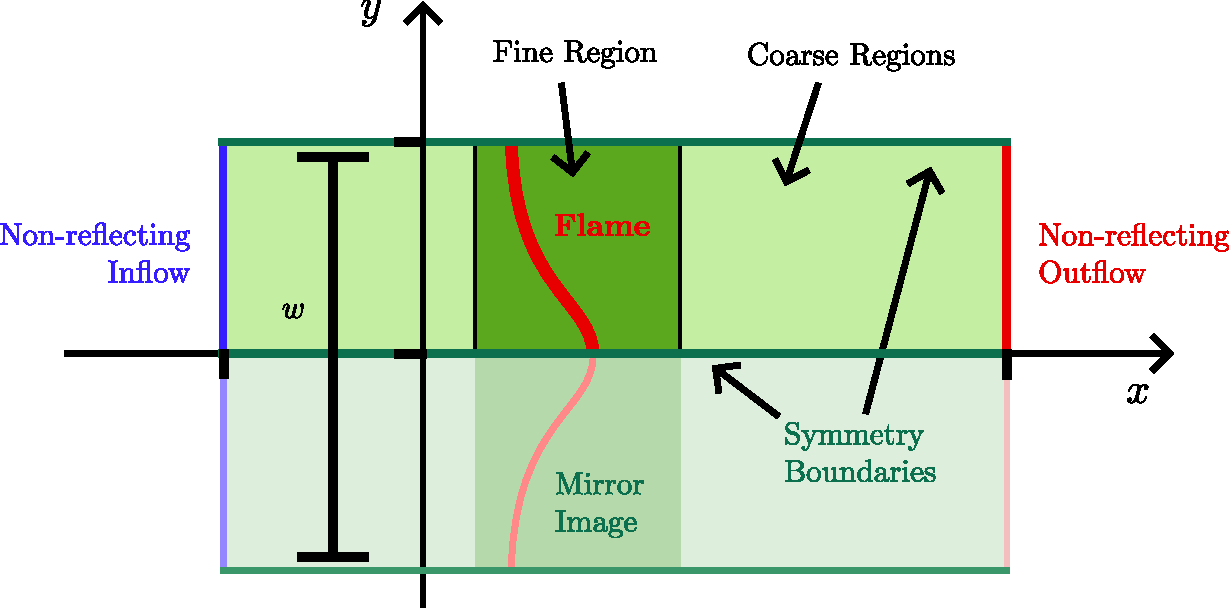
\includegraphics[scale=0.6]{assets/imgs/DNS-computational-domain.pdf}
\caption{DNS COMPUTATIONAL DOMAIN}
\label{fig:DNS-domain}
\end{figure}
    
    